\documentclass[12pt,a4paper]{article}
\usepackage[utf8]{inputenc}
\usepackage{amsmath}
\usepackage{graphicx}
\usepackage{subfig}
\usepackage{float}
\usepackage{lipsum}
\usepackage[super]{nth}
\usepackage{hyperref}
\begin{document}
\large
\title{Major Project}
\maketitle
\author{Nrupesh Surya U, Abhinav Basu, Sarvesh Borkar, Ashwani Singh}


%--------------------------------------------------------------------------------
\section*{Abstract}
The problem statement requires a working model for forecasting
the spread of COVID-19 in the United States of America. The data was collected from Official government sources 
as well as private giants such as Google and Apple who collect mobility
data. The dataset collected ranges from March 2020 to April 2021 and contains
27 features which are all time-series data.   
%--------------------------------------------------------------------------------
%--------------------------------------------------------------------------------
\section*{Introduction}
The COVID-19 pandemic, also known as the coronavirus pandemic, is an ongoing global pandemic of coronavirus disease 2019 (COVID-19) caused by severe acute respiratory syndrome coronavirus 2 (SARS-CoV-2).
\\\\
Time series forecasting has been extensively studied using classical 
statistical models like ARIMA, SARIMA and recently developed FBProphet by Facebook.
\\
Time series forecasting can be divided into univariate and multivariate. We will
be focusing on multivariate time series forecasting. 
\\\\
Our goal is to forecast New cases for the United States of America. For this, we transformed our 
time series dataset to a suitable supervised machine learning problem. 

\section*{Data Collection}
Data was collected from the Our World in Data \href{https://ourworldindata.org/coronavirus-source-data}{website}. 
The data collected from this source included new cases, deaths, testing, vaccinations. 
The data had different start dates so the data was merged by removing the missing data and 
thus the time series starts from March, 2020.   
\\\\
Mobility data was collected for the region which had data regarding the movement of people.
The Google mobility data contained features such as residential percent change from baseline,
parks percent change from baseline and so on. These data are location centric which was different
from Apple's Mobility data. This one contained just 3 features : driving, walking and transit which 
were focused just on the means of transportation. 

\section*{Exploratory Data Analysis}
The COVID-19 Cases and Death Counts are visualized in the following plots.
\begin{figure}[H]
    \centering
    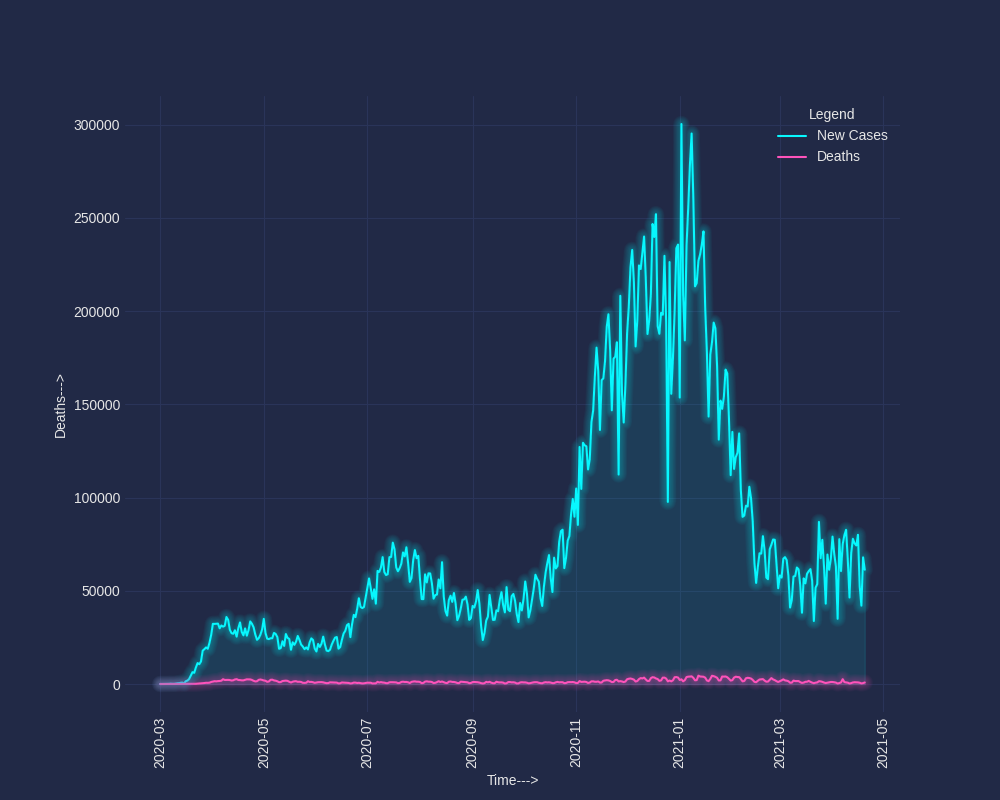
\includegraphics[width=0.75\textwidth,height=75mm]{images/usa/deaths and cases.png}
    \caption{New Cases and Deaths in USA}
\end{figure}


Figure 1 illustrates the fatality rate and infection rate of COVID-19
and gives a glimplse on exponential growth.

The testing data for the entire country is shown below.
\begin{figure}[H]
    \centering
    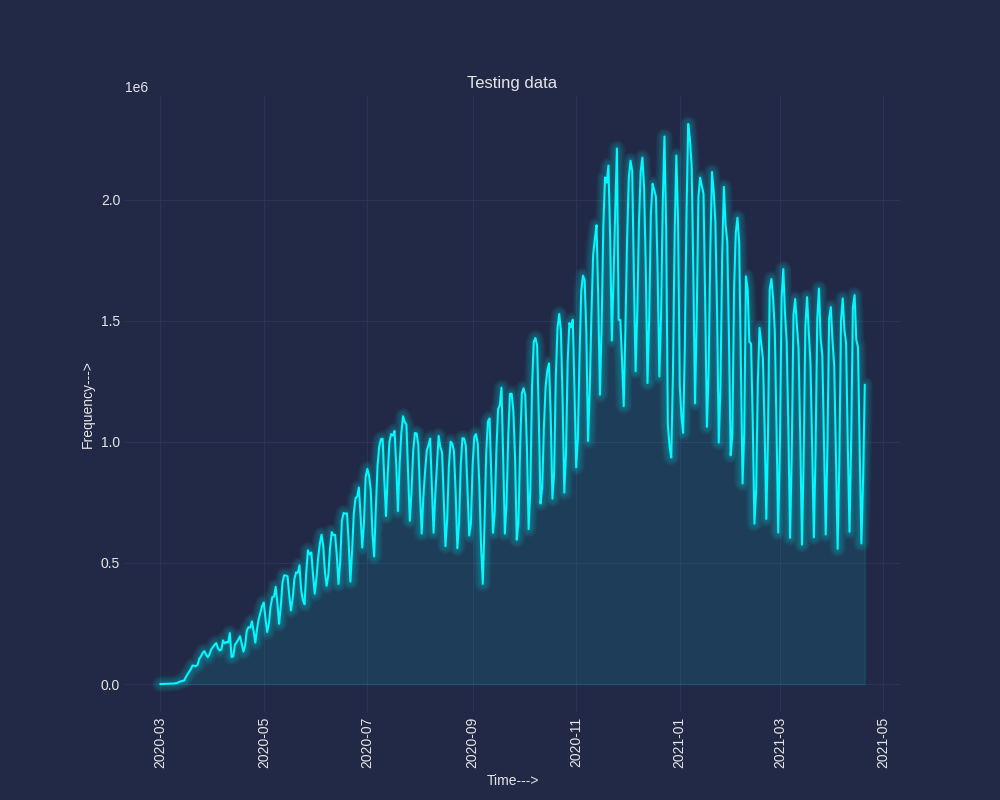
\includegraphics[width=0.75\textwidth,height=75mm]{images/usa/tests.png}
    \caption{Tests in USA}
\end{figure}
Google Mobility contains data which is location
centric such as parks, grocery stories and so on. 
\begin{figure}[H]
    \centering
    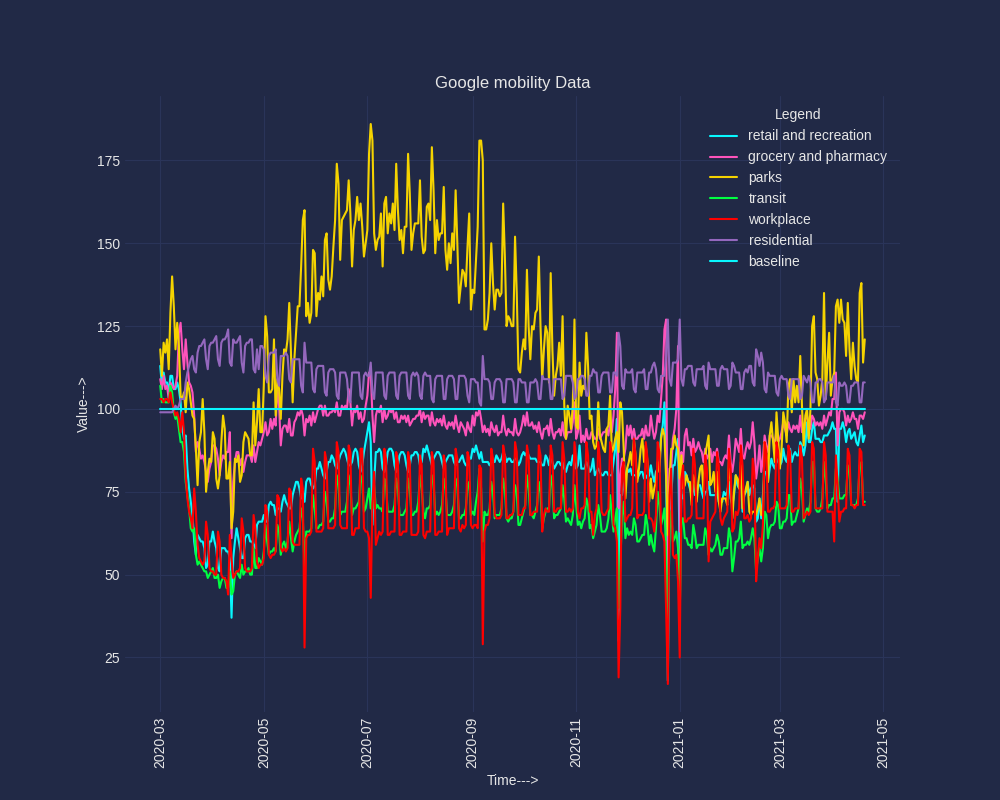
\includegraphics[width=0.6\textwidth,height=60mm]{images/usa/google.png}
    \caption{Google Mobility data}
\end{figure}
From Figure 3, we notice that almost all numbers are down from baseline
except residential, which means people have been staying at home. The other 
exception is Parks where people seemingly visited more than usual after 
lockdown which also plummets down soon enough embracing the second wave.
\\
Meanwhile Apple mobility is more transport oriented and contains driving, walking and transit data which 
shows similar trends.
\begin{figure}[H]
    \centering
    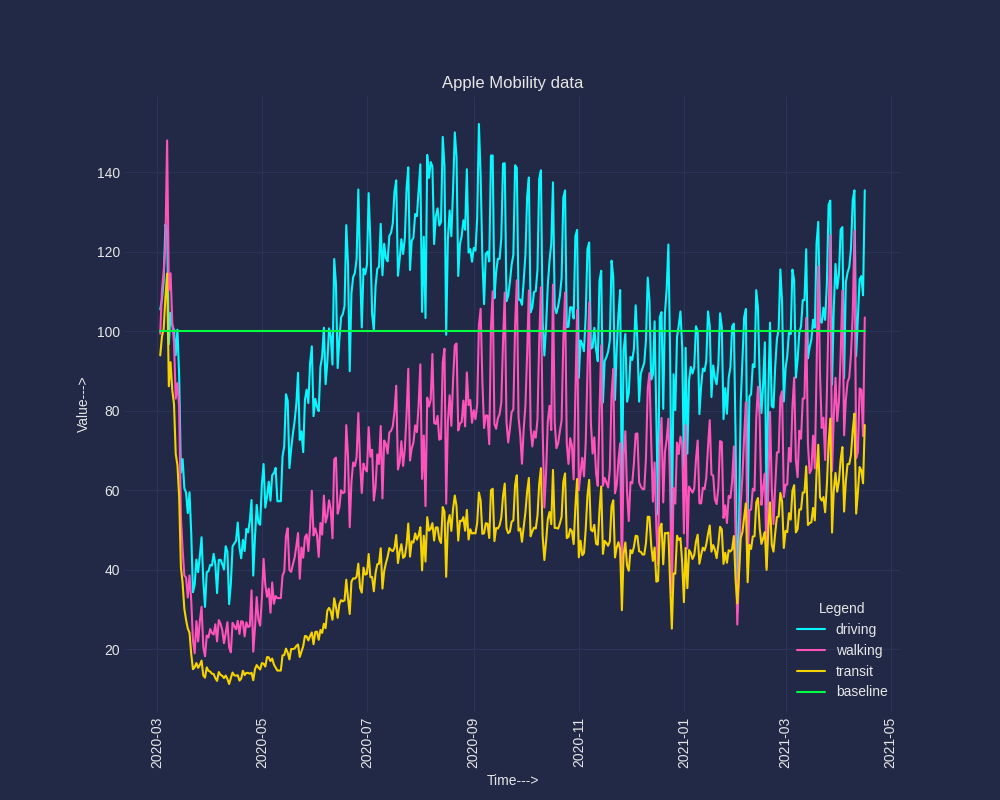
\includegraphics[width=0.6\textwidth,height=60mm]{images/apple.png}
    \caption{Apple Mobility data}
\end{figure}
The Stringency Index is a metric being used by the Oxford COVID-19 Government Response Tracker.
It is a number from 0 to 100 that reflects these indicators. A higher index score indicates a higher level of stringency.
\begin{figure}[H]
    \centering
    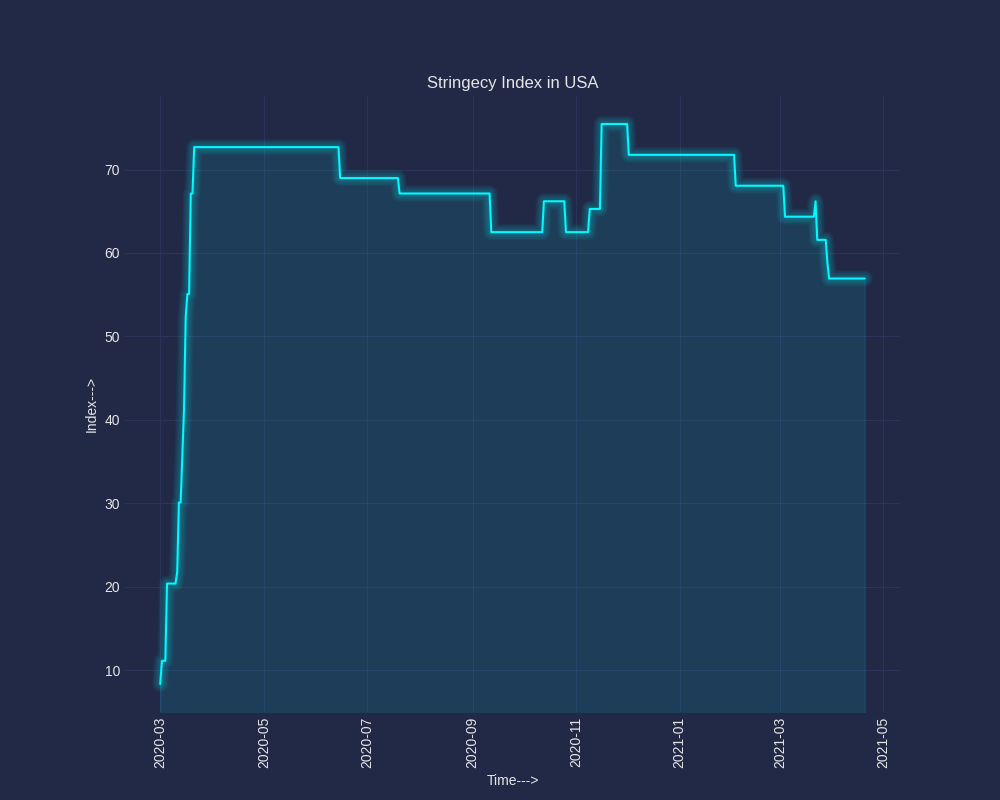
\includegraphics[width=0.6\textwidth,height=60mm]{images/usa/stringecy index.png}
    \caption{Stringency Index of USA}
\end{figure}
USA began its vaccination program at the end of last year. The following plot shows us 
people who got a vaccine shot as well as people who got fully vaccinated. 
\begin{figure}[H]
    \centering
    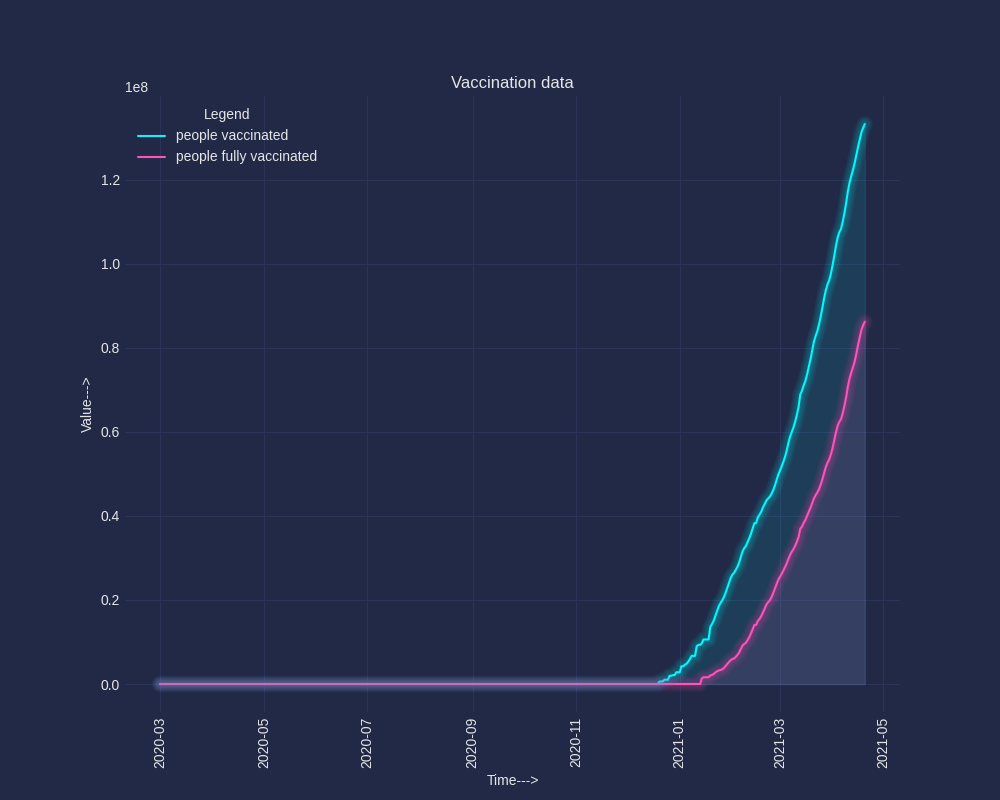
\includegraphics[width=0.6\textwidth,height=60mm]{images/usa/vaccination.png}
    \caption{COVID-19 vaccinations in USA}
\end{figure}
\section*{Data Representation}
To convert this time series dataset into a supervised machine 
learning problem we use a sliding window method. 
\begin{figure}[H]
    \centering
    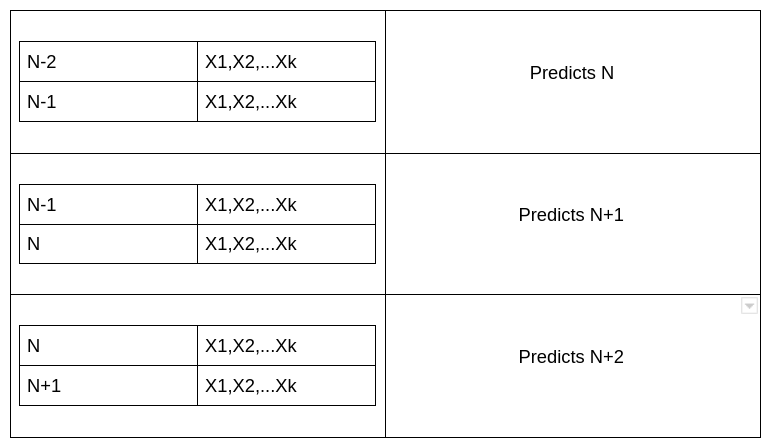
\includegraphics[width=0.6\textwidth,height=60mm]{images/sliding_window.png}
    \caption{Sliding Window with window length 2 which predicts 1 day ahead}
\end{figure}
For instance, in Figure 5, we predict the outcomes of day N using the features of the previous
2 days. 
\\
We need to extend this method to predict days further ahead in the future.
\begin{figure}[H]
    \centering
    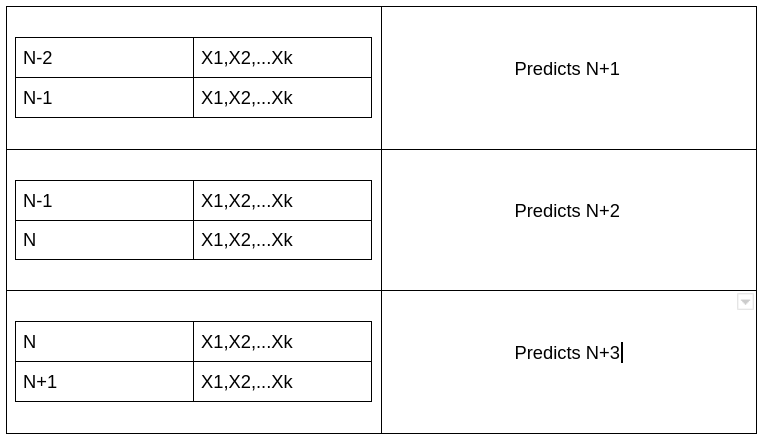
\includegraphics[width=0.6\textwidth,height=60mm]{images/sliding_window_2.png}
    \caption{Sliding Window with window length which predicts 2 days ahead}
\end{figure}
Thus, the window length becomes a hyperparameter which can be tuned further.

\section*{Data Preprocessing}
The entire dataset contained 416 data-points from March-2020 to April-2021. The window 
length was setup to be 7. This meant we had a total of 409 data points usable since we can 
only start predicting from the 7th day. The test data consisted of the last 15 data-points and the
rest was dedicated for training.
The dataset contains 27 columns for each day in the time series.
\\\\
The data was coming from multiple sources and had different
start and end dates. Missing data was removed(only from the beginning and end dates). Data was scaled
using standard scalar from Sklearn. Transforming the data into the above-mentioned sliding-window
representation was necessary before the fitting the models.
The training and test datasets further needed transformation from a 3D matrix to a 2D matrix
which was achieved by flattening.

\section*{Models}
The Python library Sklearn was used for obtaining the models which are listed below.
\begin{itemize}
    \item Support Vector Regressor : Used for linear and non-linear classification which is 
    benefited by its use of kernel tricks to manipulate data in higher dimensional spaces. 
    Since the number of data points is greater than number of features, SVR can be a good choice for
    this problem. 
    \item ARDRegressor : Automatic Relevance Determination is a classical method
    based on Bayesian interference. It fits the weights of a regression model using an ARD prior. The weights of the regression model are assumed to be in Gaussian distributions.
    \item RandomForestRegressor : Random forest is a decision tree ensemble technique that is capable of mapping complex
    non-linear decision boundaries. It builds a large number of uncorrelated trees so as to
    reduce the amount of variance and improve the accuracy and limit overfitting.
    \item GradientBoostingRegressor : Similar to random forest, gradient boosting is also a decision tree based ensemble
    technique. The difference lies in the principle - gradient boosting uses boosting, where
    the classifiers are trained sequentially, while random forests use bagging, where classifier
    is trained in parallel with a randomised subset of data.
    \item SGDRegressor : SGD stands for Stochastic Gradient Descent where the gradient of the loss is estimated each sample at a time and the model is updated along the way with a decreasing strength schedule (aka learning rate) using 
    either L1 or L2 norm.
    \item LinearRegression : LinearRegression fits a linear model with coefficients to minimize the residual sum of squares between the observed targets in the dataset, and the targets predicted by the linear approximation.\\\\
\end{itemize}
\newpage
\section*{Results and Discussion}

\begin{table}[htb]
    \begin{tabular}{ |c|c|c|c|c|c|c| }
        \hline
         & SVM & SGD & Gradient Boosting & ARDRegressor & Random Forest & LR \\
        \hline
        1-day & 0.02852 & 0.17141 & \textbf{0.57315} & 0.47651 & 0.45382 & -1.29193 \\
        \hline
        2-day & -0.41746 & 0.36239 & \textbf{0.62426} & 0.43697 & 0.50757 & -2.36140 \\
        \hline
        3-day & -0.36716 & 0.30102 & \textbf{0.53226} & 0.47336 & 0.38295 & -2.25311 \\
        \hline
        4-day & -0.32269 & \textbf{0.48710} & 0.24952 & 0.43253 & 0.32018 & -1.33823 \\
        \hline
        5-day & -0.60981 & \textbf{0.57703} & 0.45547 & 0.46390 & 0.22684 & -0.35489 \\
        \hline
        6-day & -0.88087 & 0.07318 & 0.47965 & \textbf{0.75747} & 0.03995 & -0.69944 \\
        \hline
        7-day & -1.13162 & -0.61337 & 0.40716 & \textbf{0.60604} & 0.08217 & -1.05139 \\
        \hline 
        \end{tabular}
        \caption{ $R^2$ Scores for the models with X-days future predictions}
    \begin{tabular}{ |c|c|c|c|c|c|c| }
        \hline
        & SVM & SGD & Gradient Boosting & ARDRegressor & Random Forest & LR \\
        \hline
        1-day & 0.03355 & 0.02861 & \textbf{0.01474} & 0.01808 & 0.01886 &  0.07914 \\
        \hline
        2-day & 0.04895 & 0.02202 & \textbf{0.01297} & 0.01944 & 0.01700 & 0.11607 \\
        \hline
        3-day & 0.04721 & 0.02414 & \textbf{0.01615} & 0.01819 & 0.02131 & 0.11233  \\
        \hline
        4-day & 0.04567 & \textbf{0.01771} & 0.02591 & 0.01960 & 0.02347 & 0.08074 \\
        \hline
        5-day & 0.05559 & \textbf{0.01461} & 0.01880 & 0.01851 & 0.02670 & 0.04679 \\
        \hline
        6-day & 0.06495 & 0.03200 & 0.01797 & \textbf{0.00837} & 0.03315 & 0.05868 \\
        \hline
        7-day & 0.07361 & 0.05571 & 0.02047 & \textbf{0.01360} & 0.03169 & 0.07084 \\
        \hline 
        \end{tabular}
        \caption{MSE Scores for the models with X-days future predictions}
    \begin{tabular}{ |c|c|c|c|c|c|c| }
        \hline
        & SVM & SGD & Gradient Boosting & ARDRegressor & Random Forest & LR \\
        \hline
        1-day & 0.14287 & 0.14301 & \textbf{0.09601} & 0.10690 & 0.10258 & 0.22666 \\
        \hline
        2-day & 0.17735 & 0.12438 & \textbf{0.08485} & 0.12130 & 0.09861 & 0.27625 \\
        \hline
        3-day & 0.17254 & 0.12772 & \textbf{0.09727} & 0.12056 & 0.11750 & 0.25645  \\
        \hline
        4-day & 0.16822 & 0.11559 & 0.12527 & \textbf{0.11499} & 0.12322 & 0.231801 \\
        \hline
        5-day & 0.19052 & \textbf{0.09778} & 0.10735 & 0.11289 & 0.13587 & 0.19765 \\
        \hline
        6-day & 0.20938 & 0.15464 & 0.10857 & \textbf{0.07941} & 0.15046 & 0.20480 \\
        \hline
        7-day & 0.22242 & 0.20788 & 0.11932 & \textbf{0.09876} & 0.14371 & 0.22403 \\
        \hline 
        \end{tabular}
        \caption{MAE Scores for the models with X-days future predictions}
\end{table}
\newpage
\begin{itemize}
    \item $R^2$ score : Best possible score is 1.0 and it can be negative (because the model can be arbitrarily worse). A constant model that always predicts the expected value of y, disregarding the input features, would get a score of 0.0.
        \begin{equation}
            R^2 = 1 - \frac{\sum_{i=1}^{n}(y_i - \tilde{y_i})^2}{\sum_{i=1}^{n}(y_i - \bar{y})^2} 
        \end{equation}
    \item MSE score : Mean Squared Error measures the average of the squares of the errors—that is, the average squared difference between the estimated values and the actual value. 
        \begin{equation}
            MSE = \frac{1}{n}\sum_{i=1}^{n}(y_i - \tilde{y_i})^2
        \end{equation}
    \item MAE score : Mean Absolute Error is a measure of errors between paired observations expressing the same phenomenon
    \begin{equation}
        MAE = \frac{1}{n}\sum_{i=1}^{n}|y_i - \tilde{y_i}|
    \end{equation}
\end{itemize}

The trends from Table 1,2 and 3 suggest that as we increase the prediction period, 
the error shoots up for most models. Gradient Boosting performs well while predicting 1-3 days ahead, while ARD perform better in the later stages and
SGD performs well in the mid-stages. 
\newpage
\begin{figure}[H]
    \centering
    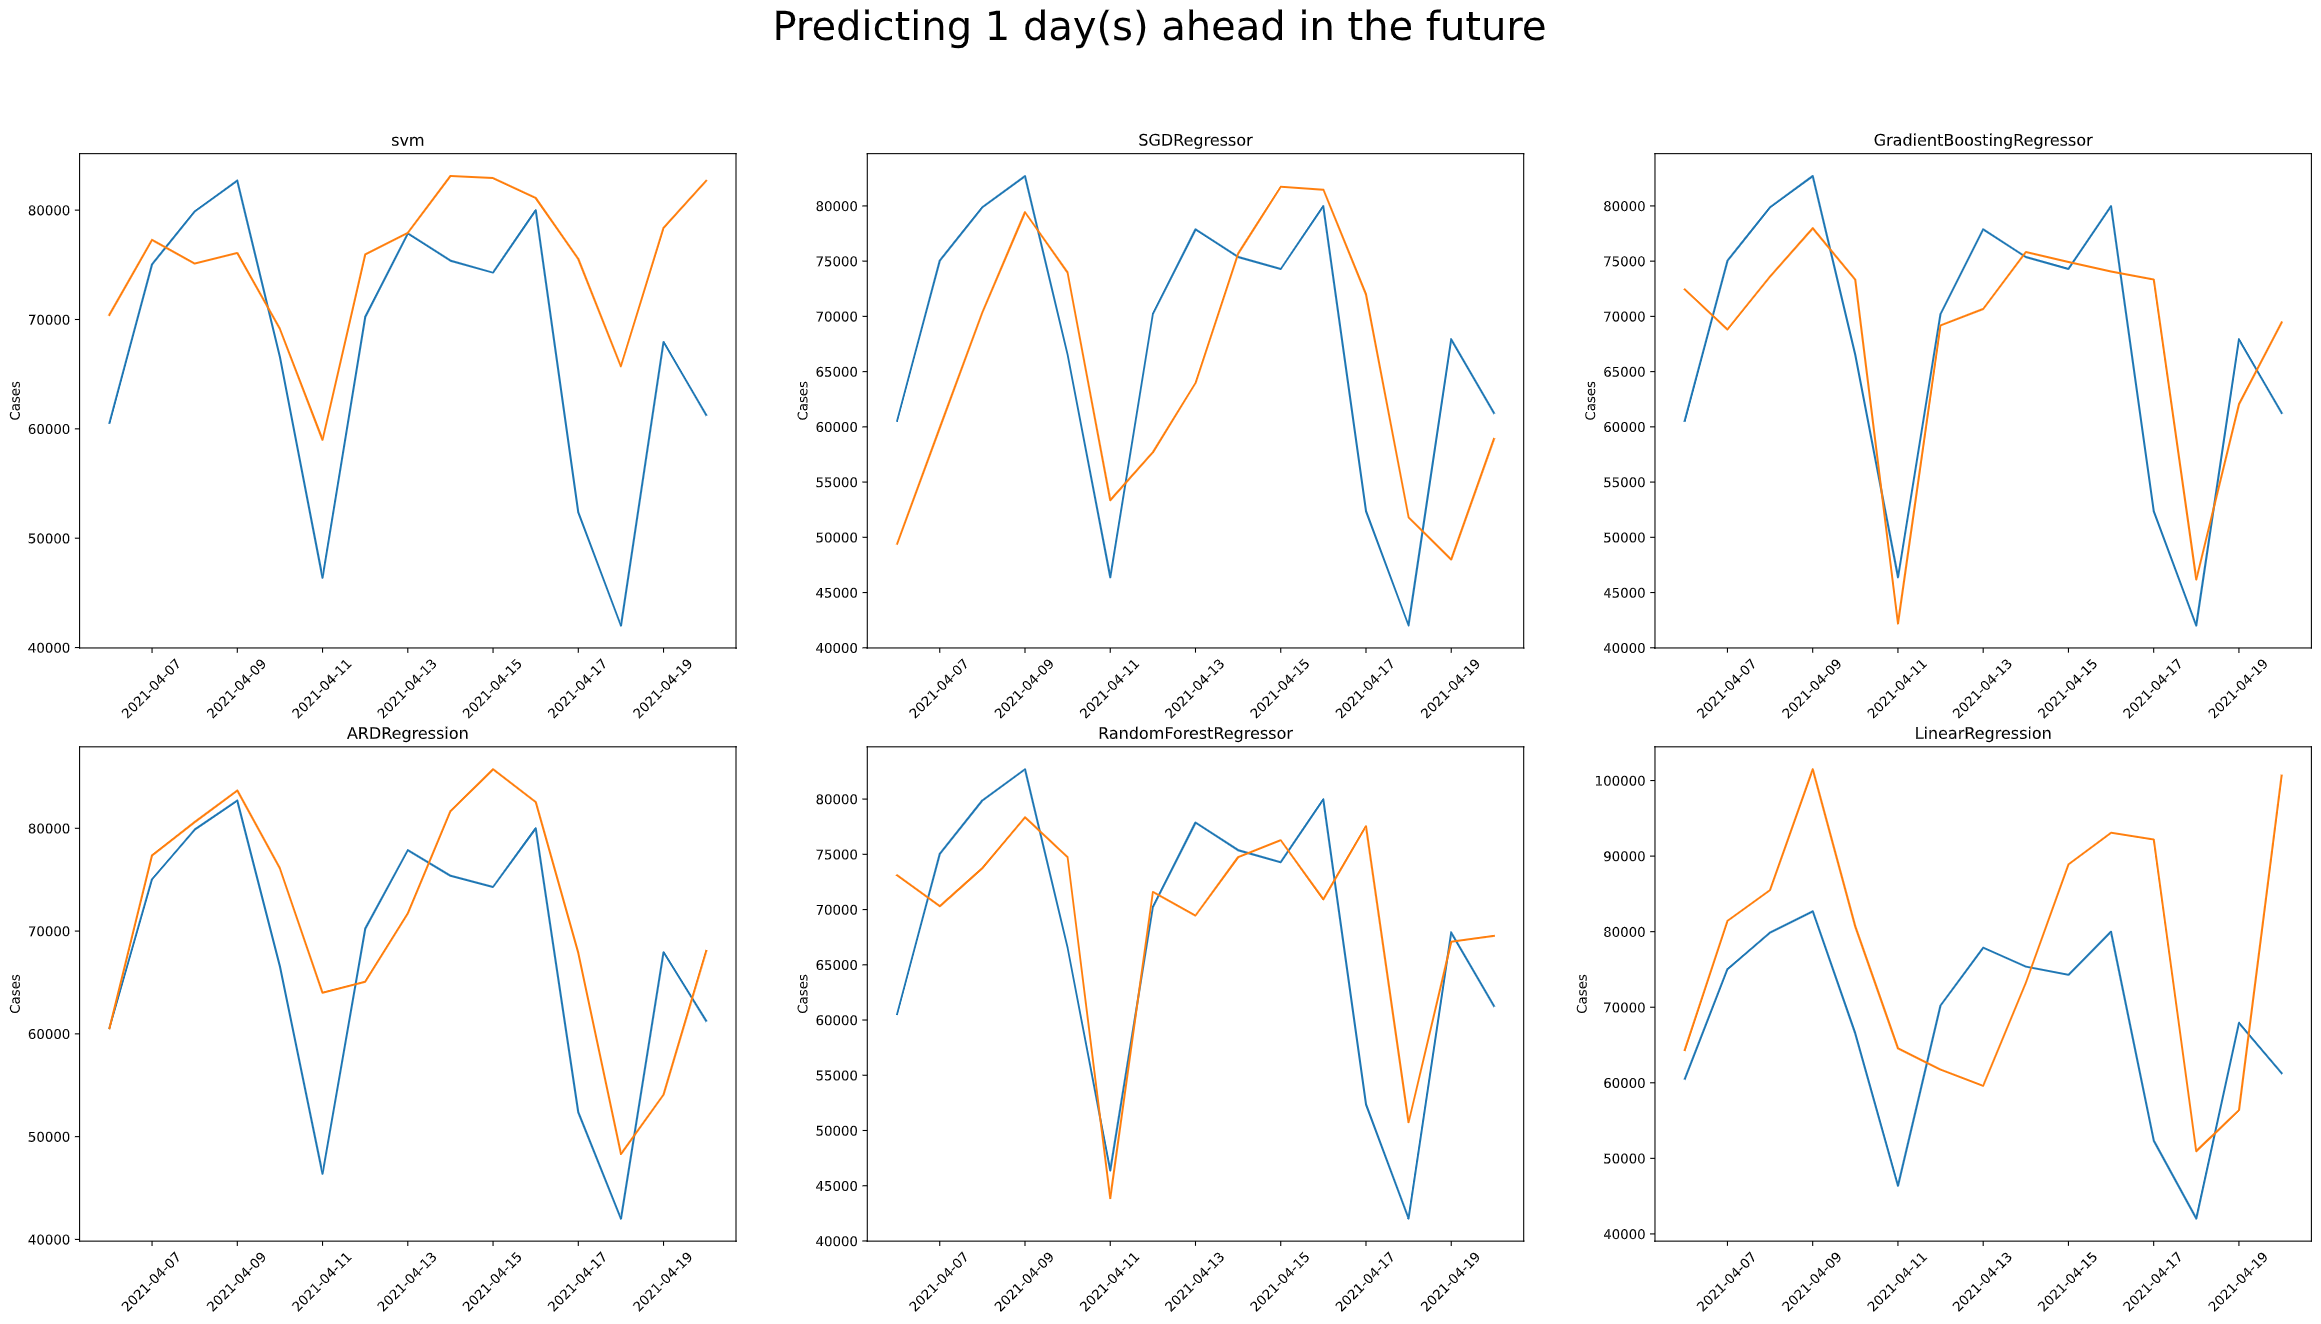
\includegraphics[width=1\textwidth,height=80mm]{images/usa/1_day.png}
    \caption{Prediction vs Test data when predicting 1 day ahead}
\end{figure}

\begin{figure}[H]
    \centering
    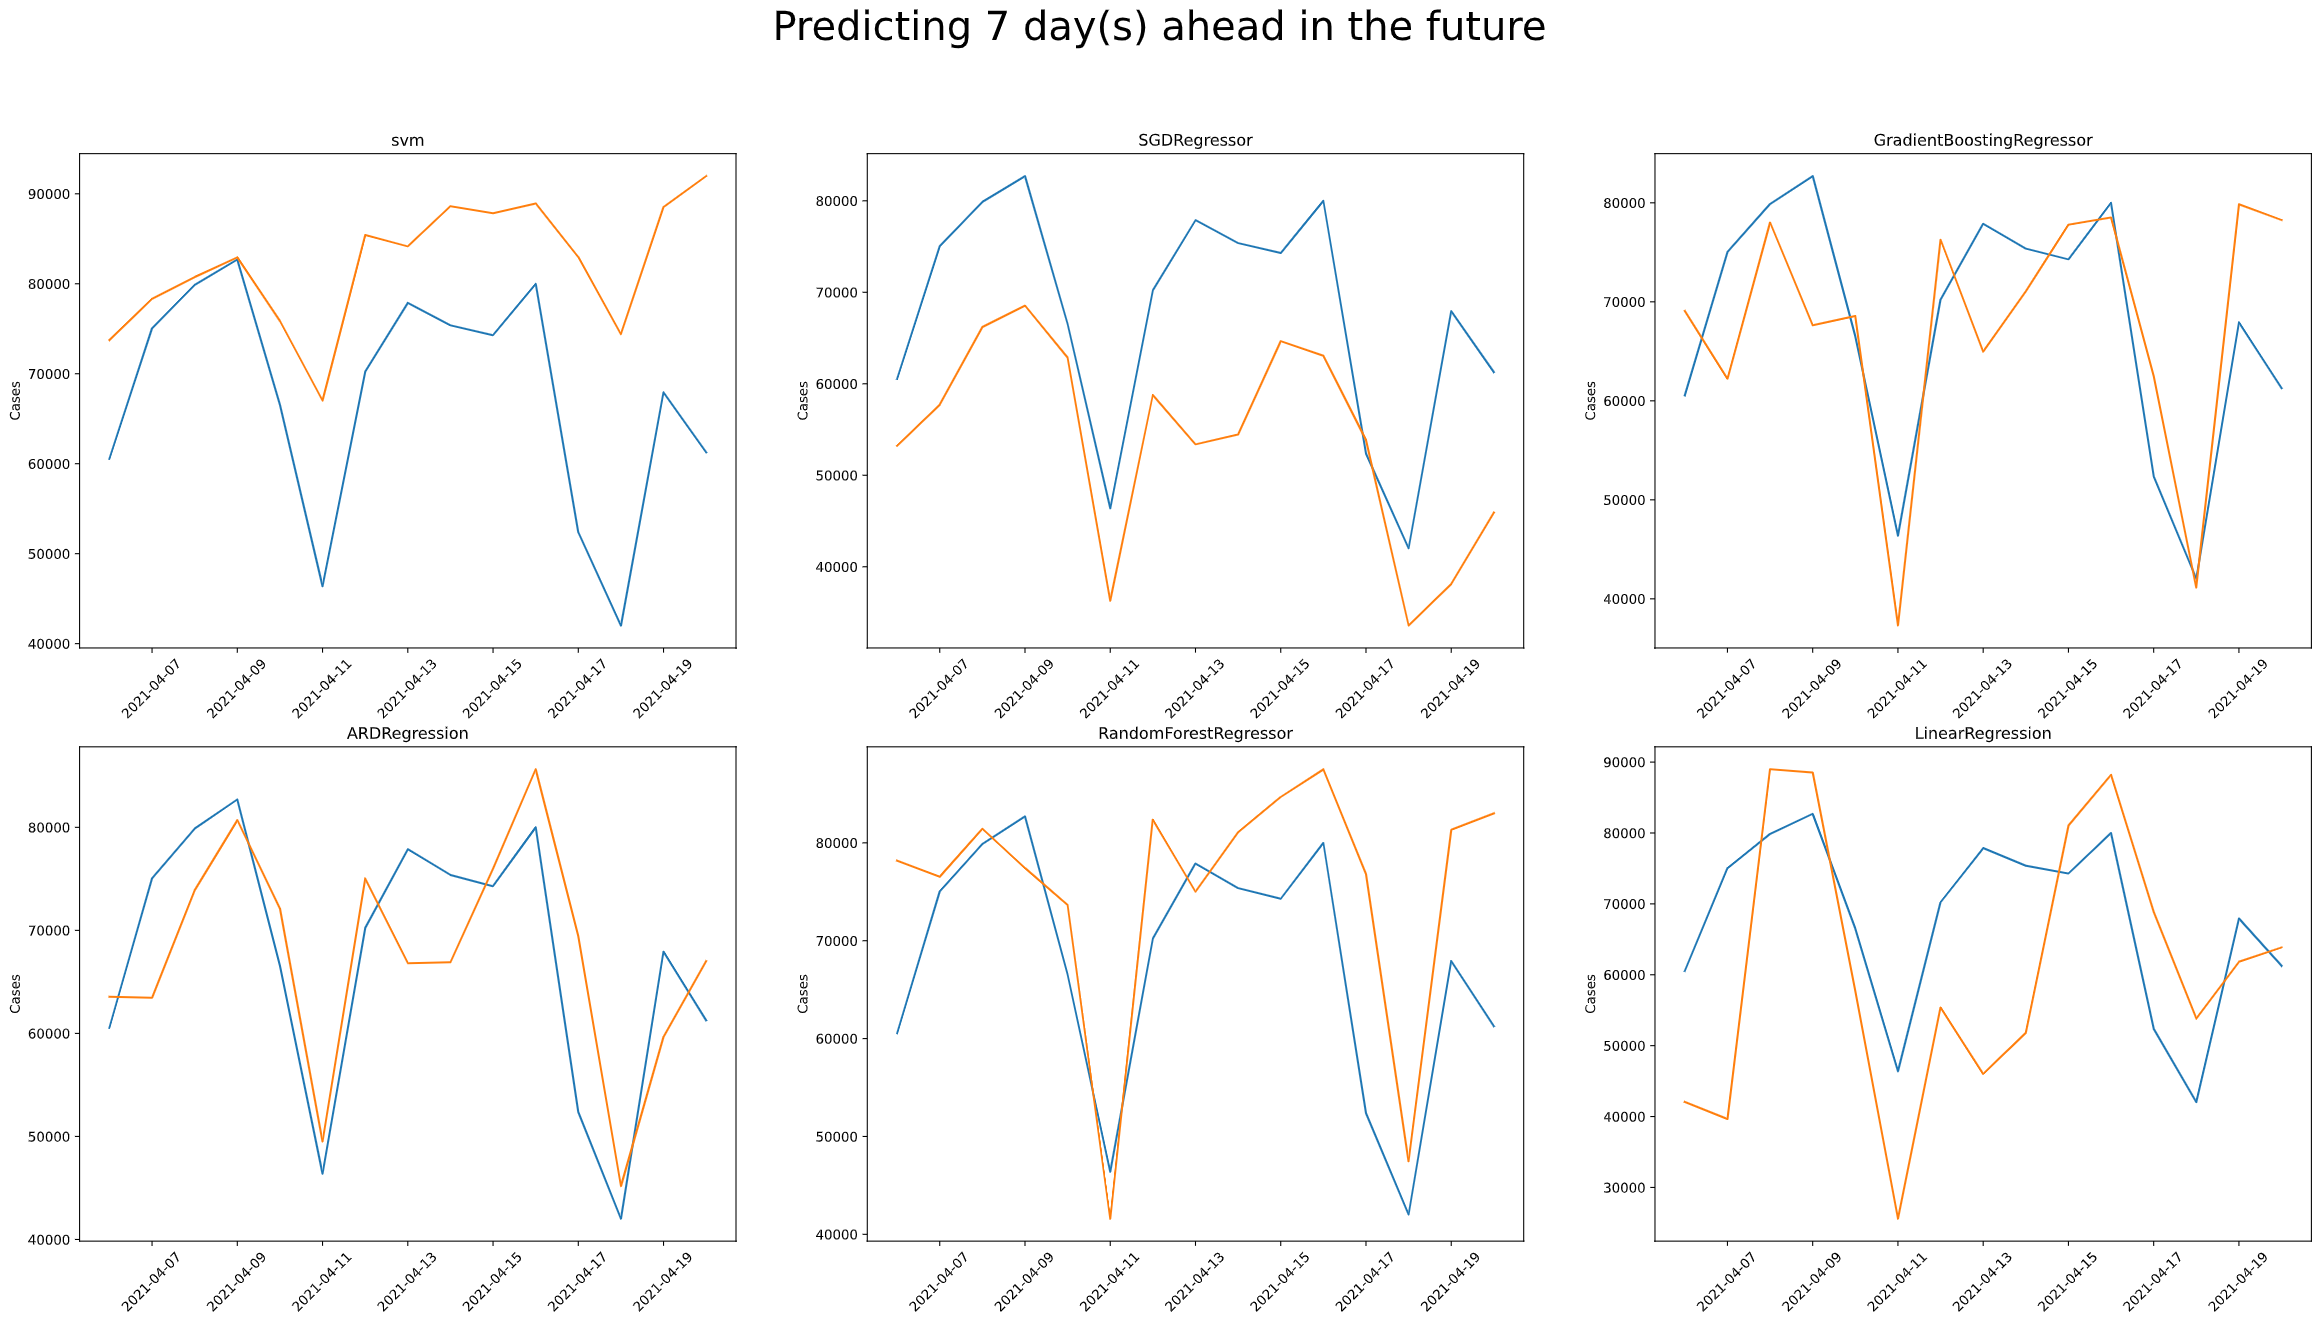
\includegraphics[width=1\textwidth,height=80mm]{images/usa/7_day.png}
    \caption{Prediction vs Test data when predicting 7 days ahead}
\end{figure}
Models which are predicting 7 days ahead seems to keep up reasonably with models which are
predicting 1 day ahead. This seems to indicate a semi-seasonality in the data.  
\section*{Comparison with other models}
Prophet is a procedure for forecasting time series data based on an additive model where non-linear trends are fit with yearly, weekly, and daily seasonality, plus holiday effects. It works best with time series that have strong seasonal effects and several seasons of historical data.
\\
This is where its limitations starts to kick in with respect to our problem.
\begin{figure}[H]
    \centering
    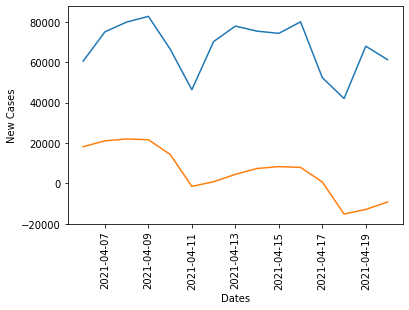
\includegraphics[width=1\textwidth,height=80mm]{images/usa/fbprophetrun.png}
    \caption{FBProphet Run for same test set}
\end{figure}
A univariate model was fitted and produced the following results. The seasonality is picked up very 
well by the model as seen with the matching peaks and troughs but that is not enough in this case. It even goes ahead
and predicts negative values for New Cases at this time frame which truly shows the limiations of a 
univariate time-series model. 
\section*{Effects of Vaccination}
\begin{figure}[H]
    \centering
    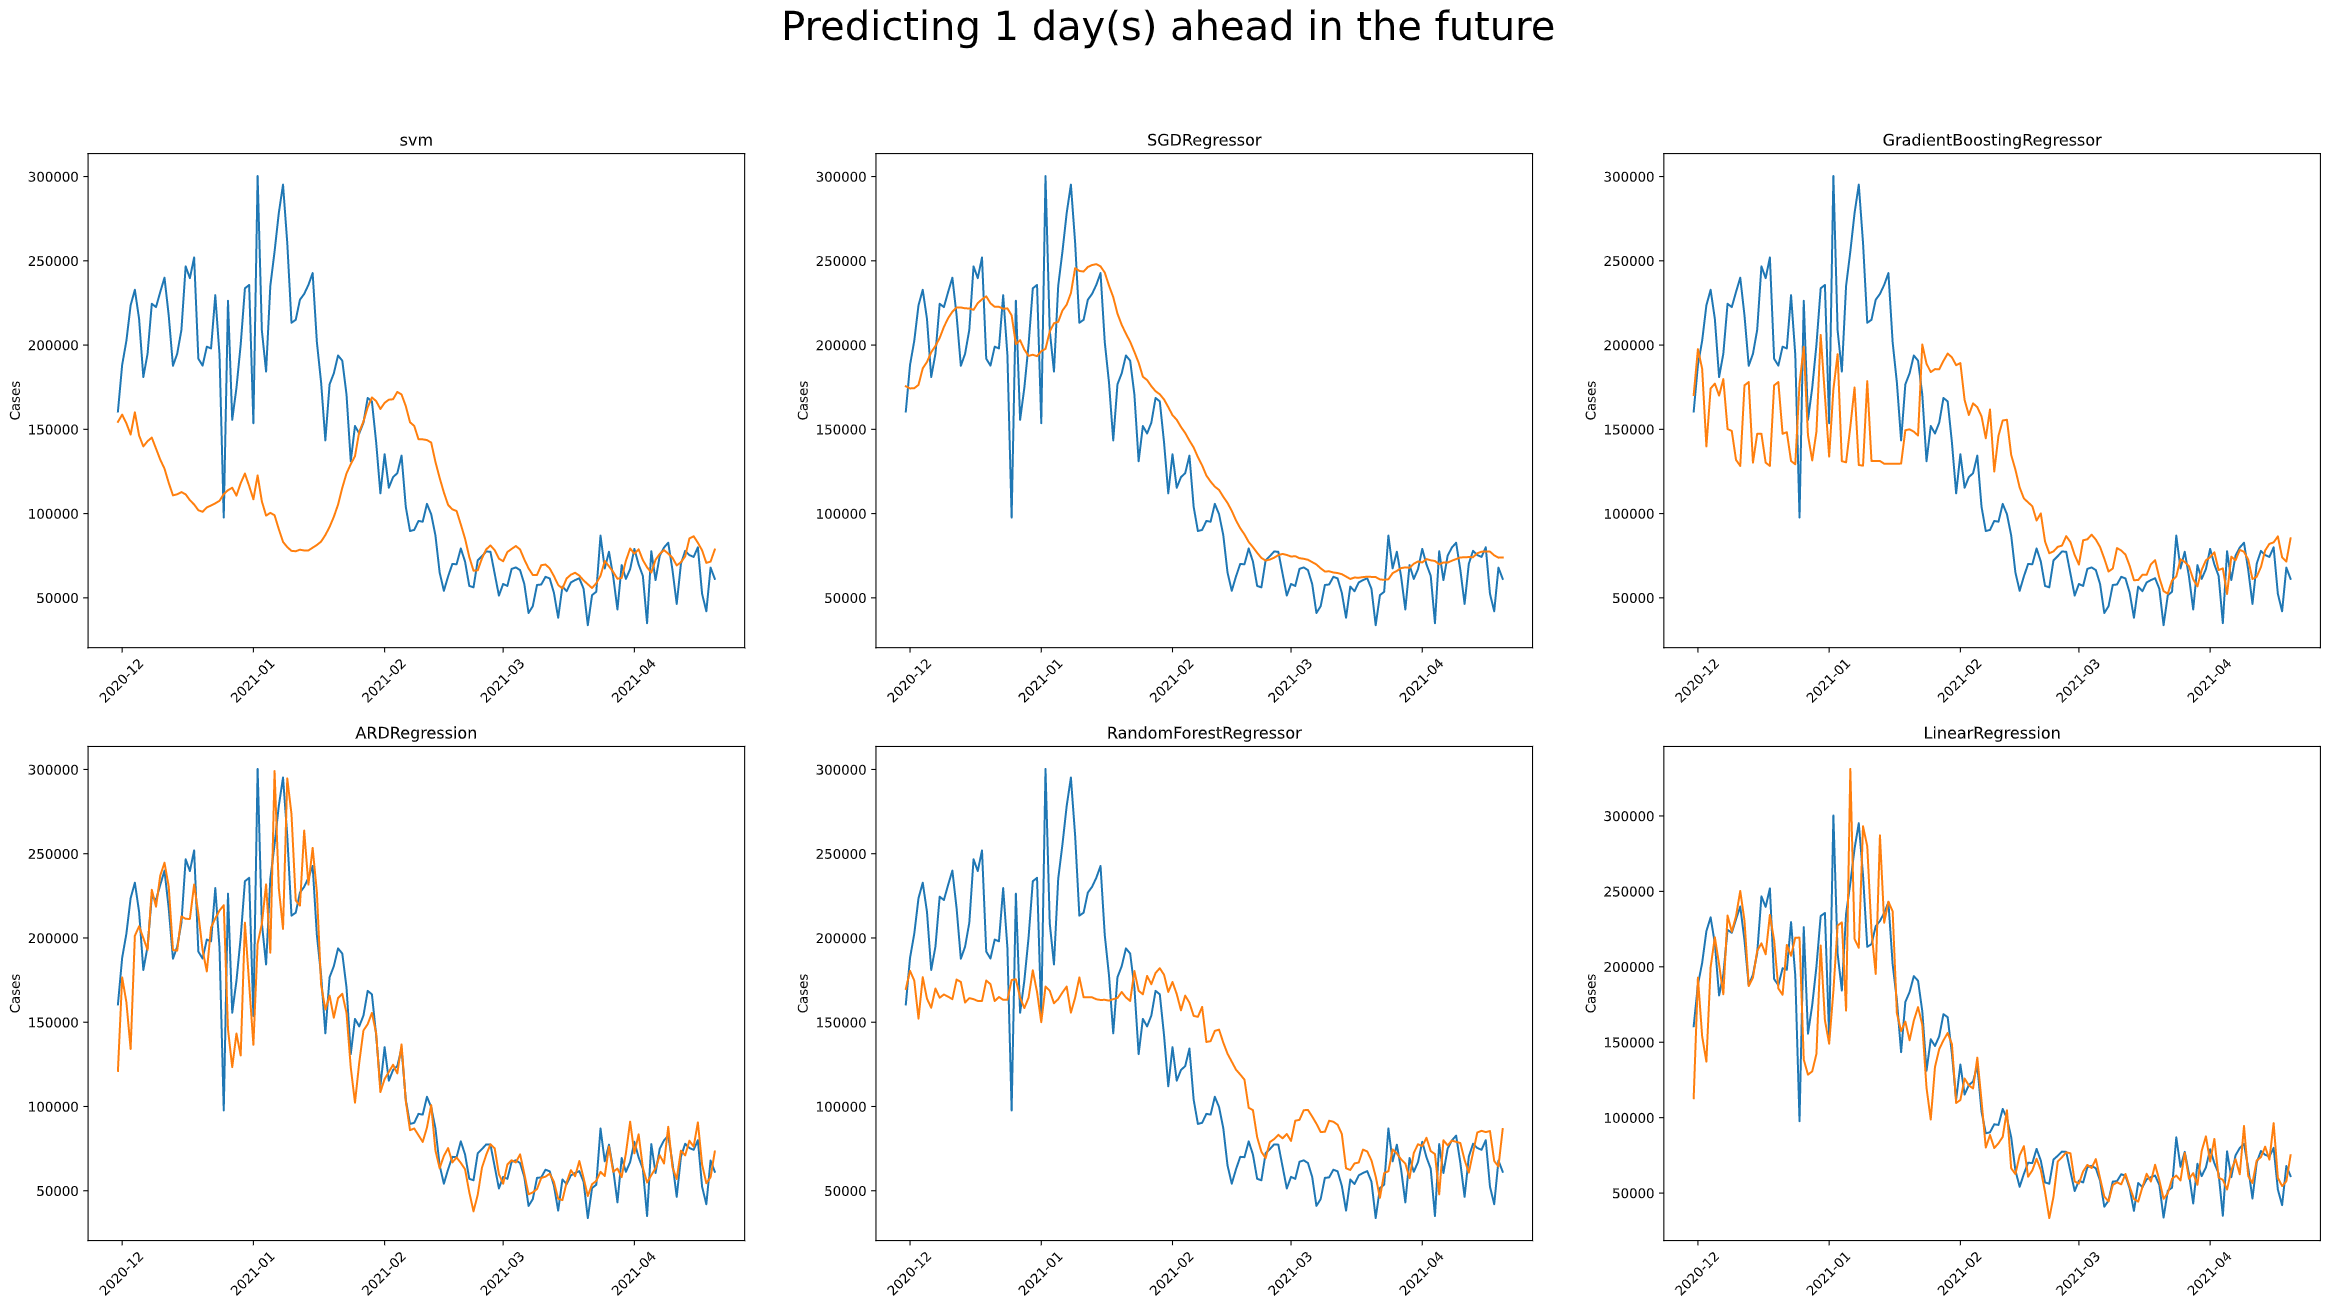
\includegraphics[width=1\textwidth,height=80mm]{images/usa/vaccination_analysis.png}
    \caption{Training till November end and forecasting without Vaccination data}
\end{figure}

In all our predictions, so far, we have incorporated vaccination data in all
of them. By removing the vaccination data (setting all the values to 0), we train out our model 
till November 2020 and forecast till April 2021. We see that the model always predicts 
lower cases till a certain threshold and then starts predicting more number of cases than the acutal numbers(in blue).
We speculate that in the first half, cases were predicted less because of the sudden spike in cases in USA(Figure 1)
which could have been caused by the US Presidential elections. But after this wave, the model constantly predicts higher case value than the 
actual data which could show a negative correlation between vaccinations and new cases.

\section*{Limitations and Future Scope}
Forecasting is a very tricky subject in itself and the main challenges we faced was 
the size of the dataset. Data is key for any Machine Learning problem but having only 416
data-points makes things way more trickier. The region of United States had a lot going on in 2020
including the Black Lives Matter movement, along with the 2020 Presidential election which caused a 
lot of spikes in the dataset. 
\\\\
This problem can further be worked upon by deep-learning models such as 
LSTM which has been well documented on its performance with time-series 
analysis. 

\section*{Conclusion}
Traditional linear models and Tree-based models have performed well to forecast
upto 7 days in the future. Although the data has sudden spikes and troughs, it is 
able to predict the semi-seasonality style of the data and does better than 
traditional univariate time series models. It is able to grasp the effects of vaccination
upto a degree but is also blinded by the second wave. With almost $30\%$ of the population 
doubly vaccinated, USA seems to be heading in the right direction for now.


\section*{Acknowledgement}
We would like to express our sincere gratitude to Prof. Ashwin Srinivasan and Prof. Tirtharaj
Dash for giving us the opportunity to do this project and also developing our fundamental
understanding of the subject.

\section*{References}
\begin{itemize}
    % \item Liu, M., Thomadsen, R. & Yao, S. Forecasting the spread of COVID-19 under different reopening strategies. Sci Rep 10, 20367 (2020). https://doi.org/10.1038/s41598-020-77292-8
    \item Dietterich T.G. (2002) Machine Learning for Sequential Data: A Review
    \href{https://doi.org/10.1007/3-540-70659-3_2}{DOI}
    \item J. Chou and T. Nguyen, "Forward Forecast of Stock Price Using Sliding-Window Metaheuristic-Optimized Machine-Learning Regression,"
     DOI : 10.1109/TII.2018.2794389
    \item Liu, M., Thomadsen, R. and Yao, S. Forecasting the spread of COVID-19 under different reopening strategies. 
      \href{https://doi.org/10.1038/s41598-020-77292-8}{DOI}
    \item Time Series Forecasting as Supervised Learning. \href{https://machinelearningmastery.com/time-series-forecasting-supervised-learning/}{machinelearningmastery}
\end{itemize}

\end{document}